% !TeX root = ../main.tex
\section{Действия групп и геометрические симметрии}

\task{55.25}{Примеры плоских фигур с заданной группой движений}
Под группой движений фигуры понимаем \emph{все} изометрии плоскости,
сохраняющие её, включая отражения.
\textbf{б) $\Z_3$.} Возьмём шесть точек на двух концентрических
окружностях разных радиусов:
\[
 A_j=2\bigl(\cos(2\pi j/3),\sin(2\pi j/3)\bigr),\quad
 B_j=\bigl(\cos(2\pi j/3+\pi/12),\sin(2\pi j/3+\pi/12)\bigr),
 \quad j=0,1,2.
\]
Центр масс этих шести точек --- начало координат, поэтому любая
симметрия фиксирует его. Разные радиусы заставляют её сохранять
каждую тройку отдельно. Допустимые вращения --- $0,2\pi/3,4\pi/3$.
Оси отражений внешней тройки имеют направления $j\pi/3$,
а внутренней --- $\pi/12+j\pi/3$; общей оси нет.
Значит полная группа симметрий этой конфигурации равна $\Z_3$.
\begin{center}
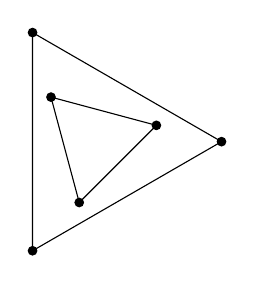
\begin{tikzpicture}[scale=.8]
\foreach \a in {0,120,240}{
 \fill (\a:2) circle (2.2pt);
 \fill ({\a+15}:1) circle (2.2pt);
}
\draw[thin] (0:2)--(120:2)--(240:2)--cycle;
\draw[thin] (15:1)--(135:1)--(255:1)--cycle;
\end{tikzpicture}
\end{center}
\textbf{г) $V_4$.} Прямоугольник, не являющийся квадратом,
имеет четыре симметрии: $e$, поворот на $\pi$ и отражения
относительно двух осей через середины противоположных сторон.
Все три неединичных элемента имеют порядок $2$;
произведение любых двух разных равно третьему.
Это группа Клейна $V_4\cong\Z_2\times\Z_2$.
Для сравнения, равносторонний треугольник имеет полную группу $S_3$
(пункт в), а равнобедренный неравносторонний треугольник --- $\Z_2$
(пункт а).
\editnote{Равносторонний треугольник даёт $\Z_3$ только при
 ограничении группы одними вращениями. Для полной группы движений
 пример в исходнике неверен.}

\task{57.1}{Орбиты векторов}
\textbf{б)} Для $G=O(n)$ орбиты --- сферы
\[\mathcal O_r=\{x\in\R^n:\|x\|=r\},\qquad r\ge0.\]
Ортогональное преобразование сохраняет норму.
Если $x,y$ имеют одну ненулевую норму, дополним $x/\|x\|$
и $y/\|y\|$ до ортонормированных базисов и переведём первый
базис во второй. Полученное ортогональное преобразование переводит
$x$ в $y$. При $r=0$ орбита состоит из нуля.

\textbf{г)} Пусть $G$ --- группа всех обратимых верхнетреугольных
матриц в фиксированном базисе $e_1,\dots,e_n$.
Орбиты равны
\[
 \mathcal O_0=\{0\},\qquad
 \mathcal O_i=\left\{\sum_{j=1}^i x_je_j:x_i\ne0\right\},
 \quad 1\le i\le n.
\]
Для вектора из $\mathcal O_i$ координаты с номерами больше $i$
остаются нулевыми, а новая $i$-я координата равна $a_{ii}x_i\ne0$.
Значит $\mathcal O_i$ инвариантно.
Покажем транзитивность. Для $x\in\mathcal O_i$ выберем матрицу
$T_x$, совпадающую с $I$, кроме $i$-го столбца, который равен $x$.
Она верхнетреугольна, имеет определитель $x_i\ne0$ и
$T_xe_i=x$. Тогда $T_yT_x^{-1}$ переводит $x$ в любой
$y\in\mathcal O_i$. Всего орбит $n+1$.

\task{57.3, а}{Стабилизатор вектора при действии $O(3)$}
Если $x=0$, его орбита --- $\{0\}$, а стабилизатор --- вся $O(3)$.
Если $x\ne0$, орбита --- сфера радиуса $\|x\|$.
Положим $u_1=x/\|x\|$ и дополним его до ортонормированного
базиса $u_1,u_2,u_3$.
Фиксирующее $x$ ортогональное преобразование фиксирует $u_1$
и сохраняет $x^\perp$: для $v\perp x$
$\langle gv,x\rangle=\langle v,g^{-1}x\rangle=0$.
В этом базисе стабилизатор имеет вид
\[G_x=\left\{\begin{pmatrix}1&0\\0&A\end{pmatrix}:A\in O(2)\right\}
 \cong O(2).\]
Блоки имеют размеры $1$ и $2$.

\task{57.7}{Действие на симметричных и эрмитовых формах}
Пусть $G=\GL(V)$, а $B$ --- множество вещественных симметричных
билинейных форм или комплексных эрмитовых форм на $V$.
Эрмитова форма в комплексном случае полуторалинейна, а не билинейна.
Зададим
\[(g\cdot b)(x,y)=b(g^{-1}x,g^{-1}y).\]
\utv{Пункт а}{Формула задаёт действие $G$ на $B$.}{
 Подстановка линейного обратимого отображения сохраняет
 симметричность, соответственно эрмитовость, формы.
 Единица действует тождественно. Далее
 \begin{align*}
 (g_1\cdot(g_2\cdot b))(x,y)
 &=b(g_2^{-1}g_1^{-1}x,g_2^{-1}g_1^{-1}y)\\
 &=b((g_1g_2)^{-1}x,(g_1g_2)^{-1}y)
 =((g_1g_2)\cdot b)(x,y).
 \end{align*}
}
\thm{Пункт б}{В обоих случаях орбиты определяются тройками
 $(p,q,r)$ неотрицательных целых чисел с $p+q+r=n$.
 Канонический вид формы --- $\diag(I_p,-I_q,0_r)$.
 Число орбит равно $\binom{n+2}{2}$.}{
 Напомним построение канонического вида. Если форма ненулевая,
 найдётся $v$ с $b(v,v)\ne0$. В вещественном случае иначе
 $b(x+y,x+y)-b(x,x)-b(y,y)=2b(x,y)$ обнуляло бы всю форму.
 В эрмитовом случае дополнительно подстановка $x+iy$
 восстанавливает мнимую часть $b(x,y)$.
 Линия $Fv$ имеет ортогональное дополнение, и
 \[V=Fv\oplus\{w:b(v,w)=0\}.
 \]
 Действительно, из любого $x$ можно вычесть подходящий кратный $v$,
 чтобы получить ортогональный ему вектор, а пересечение прямой
 с дополнением нулевое из $b(v,v)\ne0$.
 Повторяя на дополнении, диагонализуем форму; в конце остаётся
 нулевой блок. Ненулевые диагональные значения вещественны,
 и масштабированием базисных векторов они приводятся к $1$ или $-1$.

 Докажем неизменность чисел. Для указанного диагонального вида
 максимальная размерность подпространства, на котором форма
 положительно определена, равна $p$.
 Она не может превосходить $p$: подпространство большей размерности
 пересекло бы ненулевым образом координатное подпространство
 отрицательного и нулевого блоков размерности $n-p$,
 где положительных значений нет.
 Аналогично максимальная отрицательная размерность равна $q$.
 Эти характеристики сохраняются при обратимой замене переменных;
 $r=n-p-q$ тоже сохраняется.
 Две формы с одинаковыми тройками имеют один канонический вид,
 поэтому лежат в одной орбите.
 При фиксированном $p$ число вариантов $q$ равно $n-p+1$.
 Итого $\sum_{p=0}^n(n-p+1)=(n+1)(n+2)/2$.
}
\editnote{Для \emph{комплексных симметричных билинейных} форм
 орбиты действительно определяются только рангом и их $n+1$:
 любой ненулевой коэффициент имеет комплексный квадратный корень.
 Но в задаче речь об эрмитовых формах. Замена вектора на $cv$
 умножает $b(v,v)$ на $|c|^2$ и не меняет его знак.
 Ответ $n+1$ из исходника здесь неверен.}

\task{57.14, б}{Стабилизатор вершины икосаэдра}
Пусть $G$ --- группа вращений правильного икосаэдра, $v$ --- вершина.
Вращение, фиксирующее $v$, фиксирует центр $O$ и ось $Ov$.
Пять соседних с $v$ вершин лежат в плоскости, перпендикулярной
этой оси, и образуют правильный пятиугольник.
Допустимы ровно повороты вокруг оси на углы $2\pi j/5$,
$j=0,1,2,3,4$. Каждый из них сохраняет весь икосаэдр.
Поэтому $G_v\cong\Z_5$ и $|G_v|=5$.
Ось проходит через $v$ и противоположную вершину;
через центр противоположной грани она не проходит.

\task{57.13}{Группы симметрий правильных многогранников}
\textbf{а) Полная группа движений тетраэдра.}
Действие на четырёх вершинах задаёт гомоморфизм $G\to S_4$.
Он инъективен: изометрия, фиксирующая четыре аффинно независимые
точки в $\R^3$, тождественна.
Любая перестановка вершин реализуется изометрией.
Чтобы это обосновать, поместим центр в начало координат и обозначим
радиус-векторы вершин $v_1,\dots,v_4$.
Их единственная линейная зависимость --- $v_1+\cdots+v_4=0$,
а скалярные произведения зависят только от того,
совпадают ли индексы. Поэтому отображение
$v_i\mapsto v_{\sigma(i)}$ корректно продолжается до линейного
отображения пространства и сохраняет скалярное произведение.
Это требуемая ортогональная симметрия. Итак, $G\cong S_4$.

\textbf{б) Группа вращений куба.}
Правильный ответ --- $G\cong S_4$.
Куб с вершинами $(\pm1,\pm1,\pm1)$ имеет $24$ вращения:
его ортогональные симметрии переставляют три пары противоположных
граней, значит задаются перестановкой координат и независимыми
сменами их знаков. Из $3!\cdot2^3=48$ таких матриц ровно половина
имеет определитель $1$.

Действие на четырёх пространственных диагоналях даёт
$\rho:G\to S_4$. Проверим ядро. Направления диагоналей можно выбрать как
\[
 v_1=(1,1,1),\quad v_2=(1,-1,-1),\quad
 v_3=(-1,1,-1),\quad v_4=(-1,-1,1).
\]
Если $g$ сохраняет каждую диагональ, то $gv_i=\varepsilon_i v_i$,
$\varepsilon_i\in\{\pm1\}$. Из единственной зависимости
$v_1+v_2+v_3+v_4=0$ следует, что все $\varepsilon_i$ одинаковы.
Значит $g=I$ или $g=-I$. Второй вариант имеет определитель $-1$
и не является вращением. Поэтому ядро тривиально.
Образ имеет $24$ элемента и равен $S_4$.
\editnote{В исходнике и в условии задачи 57.13, б в приложенном
 издании задачника ошибочно написано $A_4$.
 Группа вращений \emph{тетраэдра} изоморфна $A_4$;
 группа вращений \emph{куба} --- $S_4$.
 Поворот куба на $\pi/2$ переставляет диагонали четверным циклом,
 который нечётен. Сохранение пространственной ориентации не означает
 чётности перестановки диагоналей.}

\textbf{в) Группа вращений икосаэдра.}
Докажем $G\cong A_5$, не используя неуточнённую конструкцию
«пяти кубов» из исходника.
\lem{}{Порядок $G$ равен $60$, а классы сопряжённости имеют
 размеры $1,15,20,12,12$.}{
 Для проверки транзитивности можно использовать координаты вершин
 \[(0,\pm1,\pm\phi),\quad(\pm1,\pm\phi,0),\quad
 (\pm\phi,0,\pm1),\qquad\phi=(1+\sqrt5)/2.\]
 Циклическая перестановка трёх координат и смена знаков любых двух
 координат сохраняют этот набор и имеют определитель $1$.
 Ими вершину $(0,1,\phi)$ можно перевести в любую из $12$ вершин:
 сначала выбираем положение нулевой координаты, затем два
 ненулевых знака; знак нулевой координаты можно менять свободно.
 Поэтому группа вращений транзитивна на вершинах.
 Стабилизатор вершины имеет порядок $5$ по задаче 57.14,
 поэтому $|G|=12\cdot5=60$.

 Перечислим вращения. Через пары противоположных вершин проходят
 $6$ осей, вокруг каждой допустимы четыре неединичных поворота
 порядка $5$: всего $24$.
 Через центры противоположных граней проходят $10$ осей;
 по два поворота порядка $3$: всего $20$.
 Через середины противоположных рёбер проходят $15$ осей;
 по одному повороту на $\pi$: всего $15$.
 С единицей получаем $1+24+20+15=60$ различных элементов,
 поэтому список полон.

 Для вращения угла, отличного от $0,\pi$, коммутирующее вращение
 должно сохранять его направленную ось. Действительно,
 сохранение ненаправленной оси необходимо по её неподвижным точкам,
 а переворот оси заменяет угол на противоположный и не коммутирует
 с исходным вращением. Централизатор имеет порядок $5$ или $3$.
 Поэтому классы имеют размеры $60/5=12$ и $60/3=20$.
 Элементы порядка $5$ составляют два класса, порядка $3$ --- один.
 Все повороты на $\pi$ сопряжены: группа транзитивна на рёбрах,
 поскольку она транзитивна на вершинах, а стабилизатор вершины
 циклически переставляет её пять соседей. Следовательно,
 она транзитивна и на парах противоположных рёбер;
 сопряжение переносит соответствующую ось вращения.
 Их класс имеет размер $15$.
}
\lem{}{Группа $G$ проста.}{
 Нормальная подгруппа есть объединение классов, содержащее единицу.
 Её порядок имеет вид $1+15a+20b+12c+12d$,
 где $a,b,c,d\in\{0,1\}$, и делит $60$.
 Возможные размеры таких объединений:
 \[1,13,16,21,25,28,33,36,40,45,48,60.\]
 Только $1$ и $60$ делят $60$.
 Следовательно, собственных нетривиальных нормальных подгрупп нет.
}
Теперь построим точное действие на пяти объектах.
Для инволюции $t\in G$ централизатор имеет порядок $60/15=4$.
В $G$ нет элементов порядка $4$, так что $C_G(t)\cong V_4$.
Если $u\ne e$ принадлежит этому $V_4$, то вся подгруппа
коммутирует с $u$ и содержится в $C_G(u)$; обе имеют порядок $4$,
поэтому совпадают.
Таким образом, $15$ инволюций разбиваются на тройки,
соответствующие ровно пяти различным подгруппам $V_4$.
Сопряжение переставляет эти пять подгрупп и задаёт $\rho:G\to S_5$.
Действие не тривиально: иначе каждая такая $V_4$ была бы нормальной,
что противоречит простоте. Ядро --- нормальная подгруппа,
поэтому оно равно $\{e\}$.
Композиция $\sgn\circ\rho:G\to\{\pm1\}$ также имеет нормальное ядро.
Она не может быть инъективной, поскольку $60>2$;
значит по простоте она тривиальна. Образ $\rho$ лежит в $A_5$
и имеет $60=|A_5|$ элементов, то есть равен $A_5$.
\editnote{Формула $12\cdot5=60$ не требует деления на $2$.
 Пять кубов обычно связывают с двойственным додекаэдром;
 их использование потребовало бы отдельно доказать точность действия.}

\task{57.19}{Элемент абелевой группы фиксирует всю орбиту}
\utv{}{Если $G$ абелева, $gm_0=m_0$ и $m\in Gm_0$, то $gm=m$.}{
 Запишем $m=hm_0$. Тогда
 $gm=ghm_0=hgm_0=hm_0=m$.
 Равенство $gh=hg$ --- именно то место, где используется абелевость.
}

\task{57.38, б}{Нормализатор подгруппы сдвигов}
Пусть
\[G=\GL_2(\R),\qquad
 H=\left\{h(a)=\begin{pmatrix}1&a\\0&1\end{pmatrix}:a\in\R\right\}.
\]
Для $g=\left(\begin{smallmatrix}p&q\\r&s\end{smallmatrix}\right)$,
$\Delta=ps-qr\ne0$, прямое вычисление даёт
\[
 gh(a)g^{-1}=\frac1\Delta
 \begin{pmatrix}\Delta-pra&p^2a\\-r^2a&\Delta+rpa\end{pmatrix}.
\]
Если $g$ нормализует $H$, нижний левый элемент при $a=1$ равен нулю,
то есть $r=0$. Тогда $p,s\ne0$ и
\[gh(a)g^{-1}=h\left(\frac ps a\right).\]
При пробеге $a$ по $\R$ величина $(p/s)a$ тоже пробегает $\R$,
поэтому здесь доказано равенство $gHg^{-1}=H$, а не только включение.
Следовательно,
\[N_G(H)=\left\{\begin{pmatrix}p&q\\0&s\end{pmatrix}:
 p,s\in\R^*,\ q\in\R\right\}.\]

\task{58.7}{Расщепление класса сопряжённости при индексе $2$}
\lem{}{Подгруппа индекса $2$ нормальна.}{
 Для $g\in H$ имеем $gH=Hg=H$.
 При $g\notin H$ и левый, и правый класс не пересекаются с $H$;
 поскольку классов ровно два, оба равны $G\setminus H$.
 Поэтому $gH=Hg$ для всех $g$.
}
\utv{}{Если $[G:H]=2$ и класс сопряжённости $C$ в $G$
 содержится в $H$, то $C$ есть один класс в $H$ либо объединение
 двух классов в $H$ одинаковой мощности.}{
 Выберем $x\in C$ и $a\notin H$. Имеем $G=H\sqcup aH$,
 поэтому
 \[C=C_H(x)^{\mathrm{cl}}\ \cup\
 aC_H(x)^{\mathrm{cl}}a^{-1},\qquad
 C_H(x)^{\mathrm{cl}}=\{hxh^{-1}:h\in H\}.
 \]
 Здесь верхний индекс $\mathrm{cl}$ отличает класс от централизатора.
 Так как $H\trianglelefteq G$, второе множество --- класс
 сопряжённости $axa^{-1}$ в $H$.
 Два класса одной группы либо совпадают, либо не пересекаются.
 Сопряжение элементом $a$ является биекцией между ними,
 так что в случае двух классов их мощности одинаковы.
}

\task{58.35}{Изоморфизм $S_4/V_4\cong S_3$}
Рассмотрим подгруппу $K\le S_4$, фиксирующую точку $4$;
$K\cong S_3$. Все неединичные элементы $V_4$ двигают точку $4$,
поэтому $K\cap V_4=\{e\}$.
Для конечных подгрупп справедливо
\[|KV_4|=\frac{|K||V_4|}{|K\cap V_4|}=6\cdot4=24.\]
Формула следует из того, что у отображения
$(k,v)\mapsto kv$ каждая непустая прообразная группа пар
имеет $|K\cap V_4|$ элементов:
$k_1v_1=k_2v_2$ равносильно $k_2^{-1}k_1=v_2v_1^{-1}\in K\cap V_4$.
Таким образом, $KV_4=S_4$.
Ограничение проекции $S_4\to S_4/V_4$ на $K$
сюръективно и имеет ядро $K\cap V_4=\{e\}$.
Следовательно, $S_4/V_4\cong K\cong S_3$.

\task{Т.3}{Раскраски граней октаэдра}
\lem{Бернсайда}{Если конечная группа $G$ действует на конечном
 множестве $X$, то число орбит равно
 \[|X/G|=\frac1{|G|}\sum_{g\in G}|\Fix(g)|.\]
}{
 Посчитаем пары $(g,x)$ с $gx=x$.
 Сначала фиксируя $g$, получаем сумму в формуле.
 Фиксируя $x$, получаем $\sum_x|G_x|$.
 На орбите $\mathcal O$ все стабилизаторы имеют порядок
 $|G|/|\mathcal O|$, так что вклад орбиты равен $|G|$.
 Деление на $|G|$ даёт число орбит.
}
У октаэдра $8$ граней. Раскраска фиксируется симметрией,
если цвет постоянен на каждом цикле её перестановки граней.
При $c$ циклах число фиксированных раскрасок равно $k^c$;
использование всех $k$ цветов не требуется.

\textbf{Отождествление только по вращениям.}
Группа имеет порядок $24$, как группа вращений двойственного куба.
\begin{center}
\small\setlength{\tabcolsep}{4pt}
\begin{tabular}{l|c|c|c}
Вращение & Число & Циклы на гранях & Раскраски\\\hline
Тождественное & $1$ & $1^8$ & $k^8$\\
$\pm\pi/2$ вокруг противоположных вершин & $6$ & $4^2$ & $k^2$\\
$\pi$ вокруг противоположных вершин & $3$ & $2^4$ & $k^4$\\
$\pi$ вокруг середин противоположных рёбер & $6$ & $2^4$ & $k^4$\\
$\pm2\pi/3$ вокруг центров противоположных граней & $8$ & $1^2 3^2$ & $k^4$
\end{tabular}
\end{center}
Например, поворот вокруг оси граней фиксирует две грани на оси,
а оставшиеся шесть собирает в две тройки.
Четверть оборота вокруг оси вершин не фиксирует граней и
переставляет их двумя четвёрками.
Поворот на $\pi$ не фиксирует ни одной грани, поскольку
треугольная грань не имеет внутренней симметрии поворота на $\pi$;
все восемь граней образуют четыре пары.
По лемме Бернсайда
\[\boxed{N_{\mathrm{rot}}(k)=\frac{k^8+17k^4+6k^2}{24}.}\]

\textbf{Отождествление по всем изометриям.}
Полная группа имеет порядок $48$ и содержит также отражающие
ориентацию симметрии. Каждая из них --- композиция центральной
инверсии с одним из $24$ вращений.
Удобно отождествить грани октаэдра с вершинами куба
$(\pm1,\pm1,\pm1)$ по направлениям нормалей.
Например, инверсия меняет все три знака, а остальные симметрии
являются знаковыми перестановками координат.
Для дополнительной половины группы получаем:
\begin{center}
\small\setlength{\tabcolsep}{4pt}
\begin{tabular}{l|c|c|c}
Инверсия, умноженная на & Число & Циклы & Раскраски\\\hline
Единицу & $1$ & $2^4$ & $k^4$\\
Поворот $\pi$ вокруг оси вершин & $3$ & $2^4$ & $k^4$\\
Поворот $\pi$ вокруг оси рёбер & $6$ & $1^4 2^2$ & $k^6$\\
Поворот $\pm2\pi/3$ вокруг оси граней & $8$ & $2\,6$ & $k^2$\\
Поворот $\pm\pi/2$ вокруг оси вершин & $6$ & $4^2$ & $k^2$
\end{tabular}
\end{center}
Это можно видеть непосредственно на координатах нормалей:
инверсия после реберного полуповорота действует как
$(x,y,z)\mapsto(-y,-x,z)$ и фиксирует четыре из восьми знаковых
троек; инверсия после третичного поворота действует как
$(x,y,z)\mapsto(-y,-z,-x)$ и имеет циклы длины $2$ и $6$.
Итак,
\[\boxed{N_{\mathrm{all}}(k)=\frac{k^8+6k^6+21k^4+20k^2}{48}.}\]
\editnote{В исходнике посчитаны $12$ рёбер вместо $8$ граней.
 При буквальном понимании «самосовмещения» как любой изометрии
 применяется $N_{\mathrm{all}}$. Если в курсе под этим словом
 понимают только вращения, применяется $N_{\mathrm{rot}}$.}

\task{58.36}{Нормальная подгруппа внутри подгруппы конечного индекса}
\utv{}{Если $[G:H]=k<\infty$, то в $H$ есть нормальная в $G$
 подгруппа $N$ с $[G:N]\mid k!$.}{
 Группа $G$ действует левыми сдвигами на множестве $k$ классов $G/H$:
 $g\cdot(aH)=(ga)H$. Получаем гомоморфизм $\rho:G\to S_k$.
 Пусть $N=\ker\rho$. Тогда $N\trianglelefteq G$.
 Элемент ядра фиксирует, в частности, класс $H$, так что
 $gH=H$ и $g\in H$; следовательно, $N\le H$.
 Точнее,
 \[N=\bigcap_{a\in G}aHa^{-1},\]
 поскольку фиксация каждого $aH$ равносильна $a^{-1}ga\in H$.
 По теореме о гомоморфизме $G/N\cong\im\rho\le S_k$.
 Отсюда $[G:N]=|\im\rho|\mid k!$ по Лагранжу.
}

\task{58.37}{Подгруппа индекса, равного минимальному простому делителю}
\utv{}{Пусть $G$ конечна, $p$ --- наименьший простой делитель
 $|G|$ и $[G:H]=p$. Тогда $H\trianglelefteq G$.}{
 По задаче 58.36 существует $N\trianglelefteq G$, $N\le H$,
 такое, что $q=[G:N]$ делит $p!$.
 Оно также делит $|G|$ и равно $p[H:N]$, поэтому $p\mid q$.
 Все простые делители $q$ не меньше $p$ (поскольку $q\mid|G|$)
 и не больше $p$ (поскольку $q\mid p!$).
 Значит единственный возможный простой делитель --- $p$.
 В $p!$ этот множитель встречается ровно один раз,
 поэтому $q=p$. Отсюда $[H:N]=1$, то есть $H=N\trianglelefteq G$.
}
